\documentclass[letterpaper, 12pt]{article}

% \usepackage[showframe, margin=1in, top=0.25in, bottom=0.25in, includeheadfoot, headheight=0.5in]{geometry}
\usepackage[margin=1in, top=0.25in, bottom=0.25in, includeheadfoot, headheight=0.5in]{geometry}

\AddToHook{cmd/section/before}{\clearpage}

\usepackage[table]{xcolor}
\colorlet{listingback}{gray!20}
\definecolor{headingcolor}{RGB}{110,34,54}

\usepackage{fancyhdr}
\renewcommand{\sectionmark}[1]{\markboth{#1}{#1}}

% Used to detect whether a section is an appendix to print the right thing in the footer
\usepackage{etoolbox}
\newtoggle{inappendix}
\pretocmd{\appendix}{\clearpage\toggletrue{inappendix}}{}{}

% Save standard definitions for head and foot rules (lines separating header and footer from text)
\let\HeadRule\headrule
\let\FootRule\footrule
% Add color to the standard definitions
\renewcommand{\headrule}{\color{headingcolor}\HeadRule}
\renewcommand{\footrule}{\textcolor{headingcolor}{\FootRule}}

% IMPORTANT: This command should not be called directly. Use \preamble.
% Macro to insert the title page for each lab.
% The argument is the title of the lab.
\newcommand{\inserttitlepage}[1]
{
    \begin{titlepage}
    \centering
    
\includegraphics[scale=0.5]{images/nexus_lab_logo.png}

    \vspace*{\baselineskip}

    \textbf{\Large OpenStack Labs}

    \vspace*{\baselineskip}

    \textbf{\Large #1}
    \vspace*{\fill}
\end{titlepage}
}

% IMPORTANT: This command should not be called directly. Use \preamble.
% Macro to define header and footer for each lab.
% The argument is the title of the lab.
\newcommand{\headfoot}[1]
{
    \fancypagestyle{fancy}
    {
        \fancyhf{}
        \fancyhead[L]{\footnotesize #1}
        \fancyhead[R]{
\includegraphics[height=0.85\headheight]{images/nexus_lab_logo.png}}
        \fancyfoot[L]{%
            \footnotesize%
            \ifnum\value{section}>0%
            \iftoggle{inappendix}{Appendix \thesection: \rightmark}{Section \thesection: \rightmark}%
            \fi}
        \fancyfoot[R]{\footnotesize\thepage}
        \renewcommand{\headrulewidth}{1.5pt}
        \renewcommand{\footrulewidth}{1.5pt}
    }
}

% Macro to insert title page, define header and footer, and insert table of contents and about section for each lab.
% The argument is the title of the lab.
\newcommand{\preamble}[1]
{
    \pagenumbering{roman}
    \inserttitlepage{#1}
    \headfoot{#1}

    % Insert table of contents
    \pagestyle{fancy}
    \tableofcontents
    \clearpage

    \section*{About This Document}
    \label{sec:about_this_document}
    \begin{itemize}
        \item This document was developed by a team at the University of Tennessee at Chattanooga led by Dr. Mengjun Xie
        (\href{mailto:mengjun-xie@utc.edu}{\textbf{mengjun-xie@utc.edu}}).
        \item The development of this document was supported by a National Centers of Academic Excellence in Cybersecurity Grant (\#H98230-20-1-0351), housed at the National Security Agency.
        \item This document is licensed with a Creative Commons Attribution 4.0 International License.
    \end{itemize}
    \clearpage
}

% Macro to insert the Lab Settings page for each lab. Call after the Introduction and Objectives sections.
\newcommand{\labsettings}
{
    \section*{Lab Settings}
    \label{sec:lab_settings}
    \addcontentsline{toc}{section}{\nameref{sec:lab_settings}}
    The information in the table below will be needed in order to complete the lab.
    The task sections below provide details on the use of this information.
    \begin{table*}[htbp]
        \centering
        \begin{tabular}{|c|c|c|c|}
            \hline
            \rowcolor{gray!20} \textbf{Virtual Machine} & \textbf{IP Address} & \textbf{Account} & \textbf{Password} \\
            \hline
            \multirow{2}{*}{\texttt{workstation}} & \multirow[t]{2}{*}{\texttt{ens3: 192.168.1.21}}  & \multirow{2}{*}{\texttt{ubuntu}} & \multirow{2}{*}{\texttt{ubuntu}} \\
                                                  & \multirow[t]{2}{*}{\texttt{ens4: 172.25.250.21}} &                                  &                                  \\
            \hline
            \multirow{2}{*}{\texttt{devstack}}    & \multirow[t]{2}{*}{\texttt{ens3: 192.168.20}}    & \multirow{2}{*}{\texttt{ubuntu}} & \multirow{2}{*}{\texttt{ubuntu}} \\
                                                  & \multirow[t]{2}{*}{\texttt{ens4: 172.25.250.20}} &                                  &                                  \\
            \hline
        \end{tabular}
    \end{table*}
    \clearpage

    % IMPORTANT(lucas): If another frontmatter section ever gets placed after this, this command needs to be moved
    % to the end of that section.
    % I have placed this here and not in each lab purely for convenience and to ensure I don't forget any.
    \pagenumbering{arabic}
}

% Sans-serif font
\renewcommand{\familydefault}{\sfdefault}
\newcommand{\texttildemid}{{\raisebox{0.5ex}{\texttildelow}}}

\usepackage{enumitem}
\renewcommand{\labelenumi}{\textbf{\thesection.\arabic{enumi}.}}

% Try to forbid widows and orphans
\widowpenalty10000
\clubpenalty10000

\usepackage{graphicx}
\usepackage{hyperref}
\hypersetup{colorlinks=true,linkcolor=black,urlcolor={[named] headingcolor}}

\usepackage{sectsty}
\sectionfont{\color{headingcolor}}

% Table of Contents
\usepackage{bookmark}
\usepackage[titles]{tocloft}
\usepackage[title]{appendix}
\renewcommand{\cfttoctitlefont}{\Large\bfseries\color{headingcolor}}
\renewcommand{\cftsecfont}{\normalfont\normalsize}
\renewcommand{\cftsecpagefont}{\normalfont\normalsize}
\renewcommand{\cftdotsep}{0} % Make dots small and close together
\renewcommand{\cftsecleader}{\cftdotfill{\cftdotsep}} % Add dots after section titles
% Make dots go all the way to the page number
\renewcommand{\cftsecfillnum}[1]{{\cftsecleader}\nobreak{\cftsecpagefont #1}\cftsecafterpnum\par}

\usepackage{multirow}
\setlength{\tabcolsep}{16pt}
\renewcommand{\arraystretch}{1.1}

% For nice-looking boxes
\usepackage[most]{tcolorbox}
\usepackage{listings}
\usepackage{lstautogobble}
\lstset{
  frame=none,
  language=Bash,
  showstringspaces=false,
  basicstyle={\linespread{1.1}\footnotesize\ttfamily\selectfont},
  numbers=none,
  breaklines=true,
  breakatwhitespace=true,
  tabsize=3,
  columns=fullflexible,
  keepspaces=true,
  escapeinside={(*@}{@*)},
  literate={~}{{\texttildemid}}{1}
           {\#}{\#}{1},
  autogobble=true
}

\tcolorboxenvironment{lstlisting}
{
    spartan,
    colframe=gray!50,
    boxsep=0mm,
    left=1mm,
    right=1mm,
    top=-1mm,
    bottom=-1mm,
    colback=gray!20
}

% Hacky solution for now, would like to have just one environment and make several tcolorboxes by passing different
% colors as parameters, but that is giving errors
\makeatletter
\tcbset{
  note/.style={%
        enhanced,
        breakable,
        colback=blue!10!white,
        colframe=blue!80!white,
        attach boxed title to top left={yshift*=-\tcboxedtitleheight},
        title={#1},
        boxed title size=title,
        boxed title style={%
            sharp corners,
            rounded corners=northwest,
            colback=tcbcolframe,
            boxrule=0pt,
        },
        underlay boxed title={%
            \path[fill=tcbcolframe] (title.south west)--(title.south east)
                to[out=0, in=180] ([xshift=5mm]title.east)--
                (title.center-|frame.east)
                [rounded corners=\kvtcb@arc] |-
                (frame.north) -| cycle;
        },
    }
}
\makeatother

\makeatletter
\tcbset{
    stop/.style={%
        enhanced,
        breakable,
        colback=white,
        colback=red!10!white,
        colframe=red!80!white,
        attach boxed title to top left={yshift*=-\tcboxedtitleheight},
        title={#1},
        boxed title size=title,
        boxed title style={%
            sharp corners,
            rounded corners=northwest,
            colback=tcbcolframe,
            boxrule=0pt,
        },
        underlay boxed title={%
            \path[fill=tcbcolframe] (title.south west)--(title.south east)
                to[out=0, in=180] ([xshift=5mm]title.east)--
                (title.center-|frame.east)
                [rounded corners=\kvtcb@arc] |-
                (frame.north) -| cycle;
        },
    }
}
\makeatother

\makeatletter
\tcbset{
    tip/.style={%
        enhanced,
        breakable,
        colback=white,
        colback=green!10,
        colframe=green!70!black,
        attach boxed title to top left={yshift*=-\tcboxedtitleheight},
        fonttitle=\bfseries,
        title={#1},
        boxed title size=title,
        boxed title style={%
            sharp corners,
            rounded corners=northwest,
            colback=tcbcolframe,
            boxrule=0pt,
        },
        underlay boxed title={%
            \path[fill=tcbcolframe] (title.south west)--(title.south east)
                to[out=0, in=180] ([xshift=5mm]title.east)--
                (title.center-|frame.east)
                [rounded corners=\kvtcb@arc] |-
                (frame.north) -| cycle;
        },
    }
}
\makeatother

% The commands below define environments for colored boxes. They are used like
% \begin{notebox}
% ...
% \end{notebox}
\newtcolorbox{notebox}{note={Note}}
\newtcolorbox{stopbox}{stop={Stop}}
\newtcolorbox{tipbox}{tip={Tip}}


\begin{document}
\begin{titlepage}
    \centering
    
\includegraphics[scale=0.5]{images/nexus_lab_logo.png}

    \vspace*{\baselineskip}

    \textbf{\Large OpenStack Labs}

    \vspace*{\baselineskip}

    \textbf{\Large Lab 01: Launching an Instance}
    \vspace*{\fill}
\end{titlepage}

\fancypagestyle{fancy}
{
    \fancyhf{}
    \fancyhead[L]{\footnotesize Lab 01: Launching an Instance}
    \fancyhead[R]{
\includegraphics[height=0.85\headheight]{images/nexus_lab_logo.png}}
    \fancyfoot[R]{\footnotesize\thepage}
    \renewcommand{\headrulewidth}{0pt}
}

\pagestyle{fancy}
\tableofcontents
\clearpage

\section*{Introduction}
\label{sec:introduction}
\addcontentsline{toc}{section}{\nameref{sec:introduction}}
In this lab, you will launch an instance using the \textit{Horizon Dashboard}, launch an instance using the
\textit{OpenStack Unified CLI}, and use the \textit{OpenStack Unified CLI}.

\section*{Objectives}
\label{sec:objectives}
\addcontentsline{toc}{section}{\nameref{sec:objectives}}
\begin{itemize}[itemsep=0pt]
    \item Use the \textit{Horizon Dashboard}.
    \item Launch an instance using the \textit{Horizon Dashboard}.
    \item Use the \textit{OpenStack Unified CLI}.
    \item Launch an instance using the \textit{OpenStack Unified CLI}.
\end{itemize}
\clearpage

\section{Launching an Instance Using the Horizon Dashboard}
In this task, you will launch an instance using the \textit{Horizon Dashboard}.

\begin{enumerate}
    % TODO(lucas): Fill in lab name
    \item Navigate to \textbf{EZSetup$\rightarrow$Workspaces$\rightarrow$[Lab Name]}.
    
    \item Log into the \textbf{workstation} machine.
    \begin{enumerate}
        \item Copy the password under \textit{Password}.
        \item Click \textbf{Open} under \textit{VNC Connection}.
        \item Paste the password into the \textit{Password} field.
    \end{enumerate}

    \item A popup window will you to choose the panel setup for the first startup. Choose \textbf{Use default config}.
    Otherwise, there will be no taskbar or panel with convenient shortcuts for the terminal or web browser.

    \item If the desktop screen is larger than the window, select the options on the left-hand side of the screen,
    click the gear icon to go to the settings menu, and under \textit{Scaling Mode}, select \textbf{Remote Resizing}.

    \item Open the web browser.

    \begin{center}
    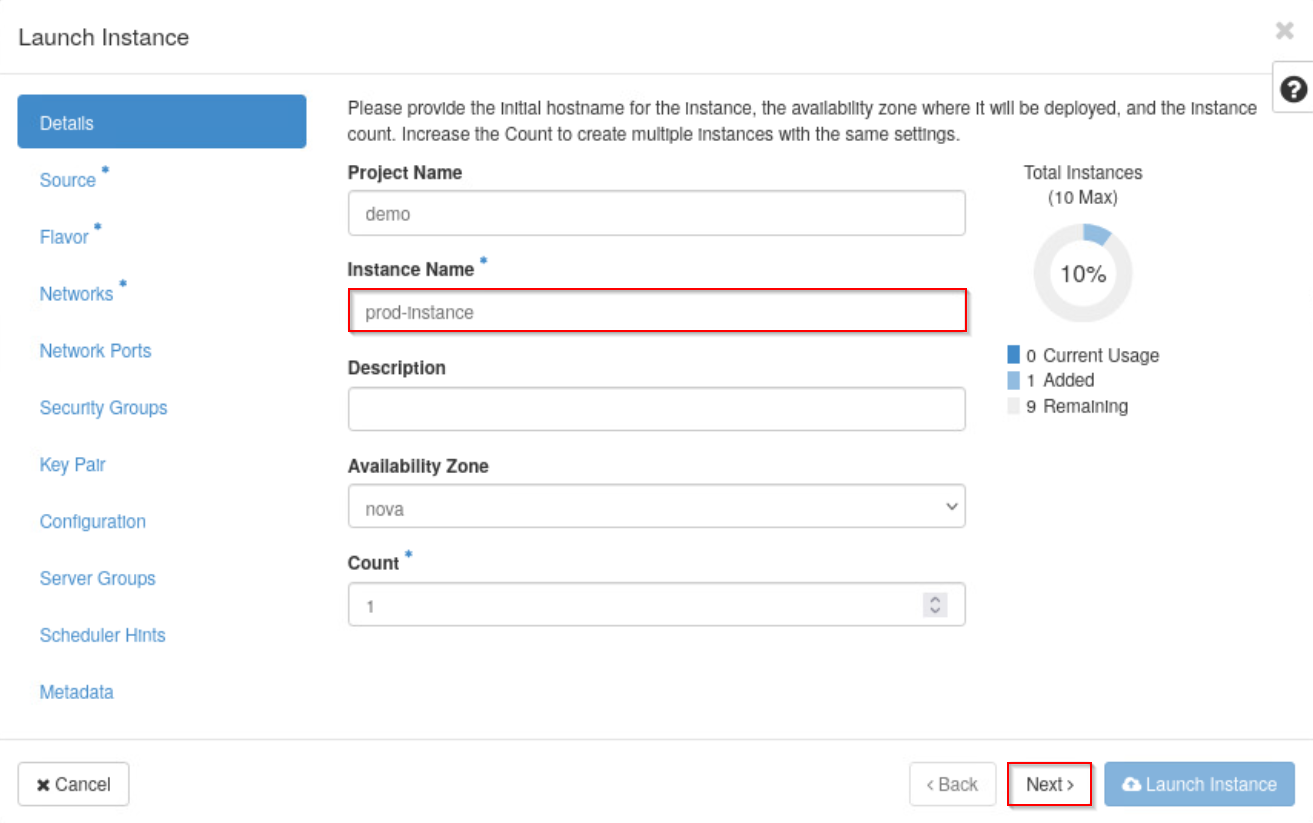
\includegraphics[scale=0.75]{images/part1/step5.png}
    \end{center}

    \item Enter the IP address of the \textbf{devstack} machine (\textbf{192.168.20.0}) into the address bar.
    
    \begin{center}
        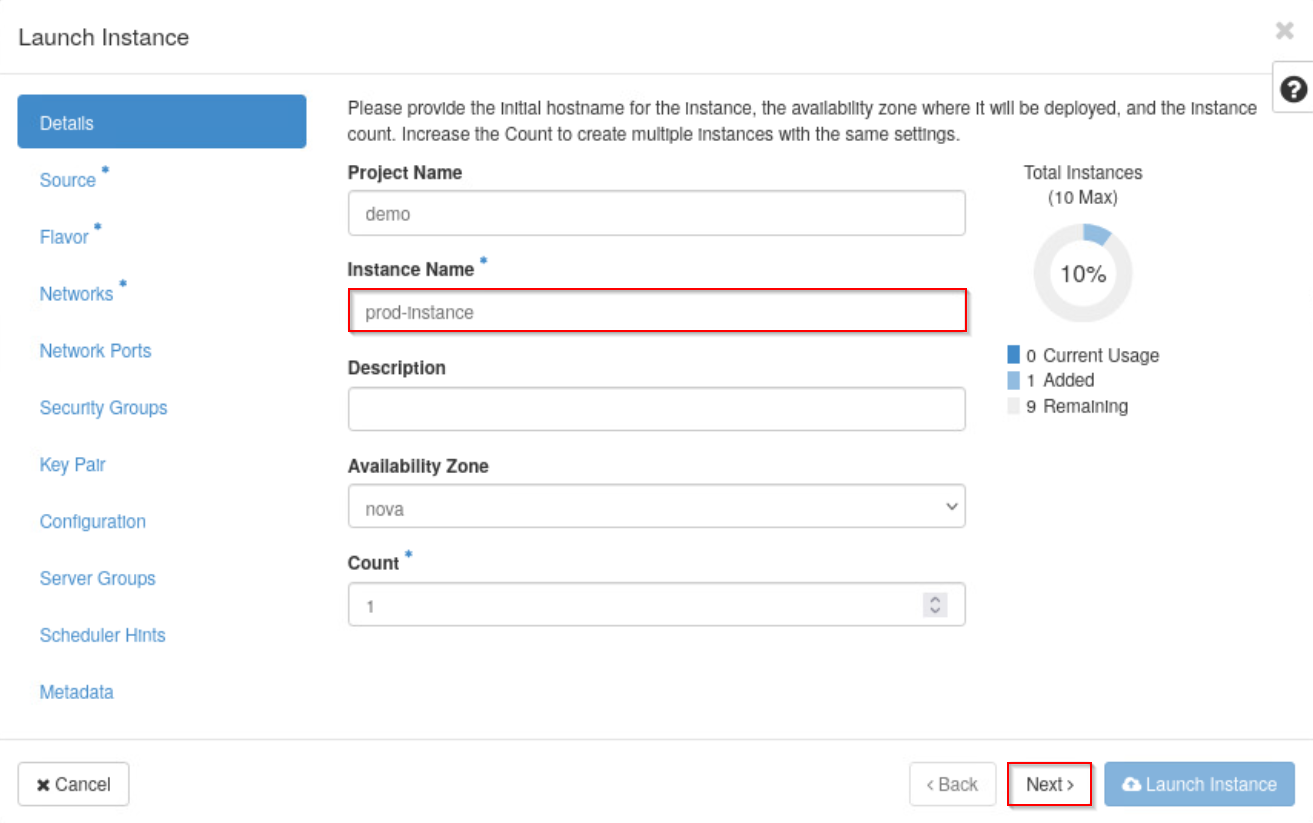
\includegraphics[width=\linewidth]{images/part1/step6.png}
    \end{center}

    \begin{tipbox}{}
        The IP address of each machine of the lab can be found by viewing the EZSetup lab page. Simply click the link
        between the machine and another object on the network (normally the cloud icon) to find the IP address for that
        interface.
    \end{tipbox}

    \item Log into the OpenStack Horizon Dashboard. The username is \textbf{admin} and the password is \textbf{secret}.
    
    \begin{center}
        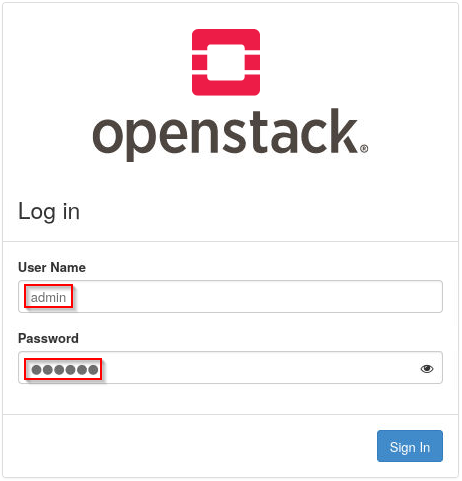
\includegraphics[scale=0.75]{images/part1/step7.png}
    \end{center}

    \item Click on the \textit{Project} tab in the top right corner of the webpage, then select \textbf{demo} as the
    project.

    \begin{center}
        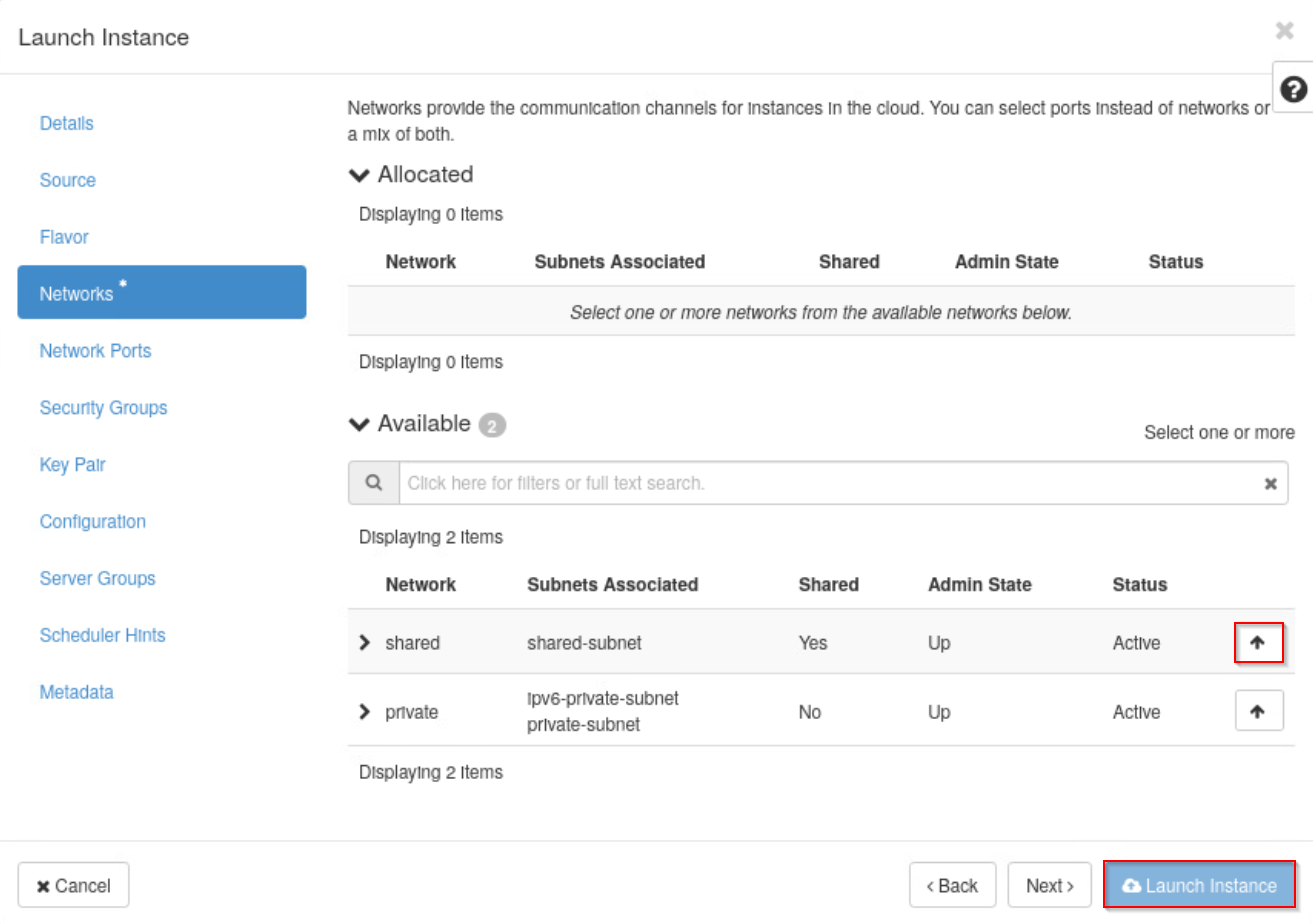
\includegraphics[scale=0.75]{images/part1/step8.png}
    \end{center}

    \item Navigate to the \textit{Instances} panel and click \textbf{Launch Instance} in the top right corner.
    
    \begin{center}
        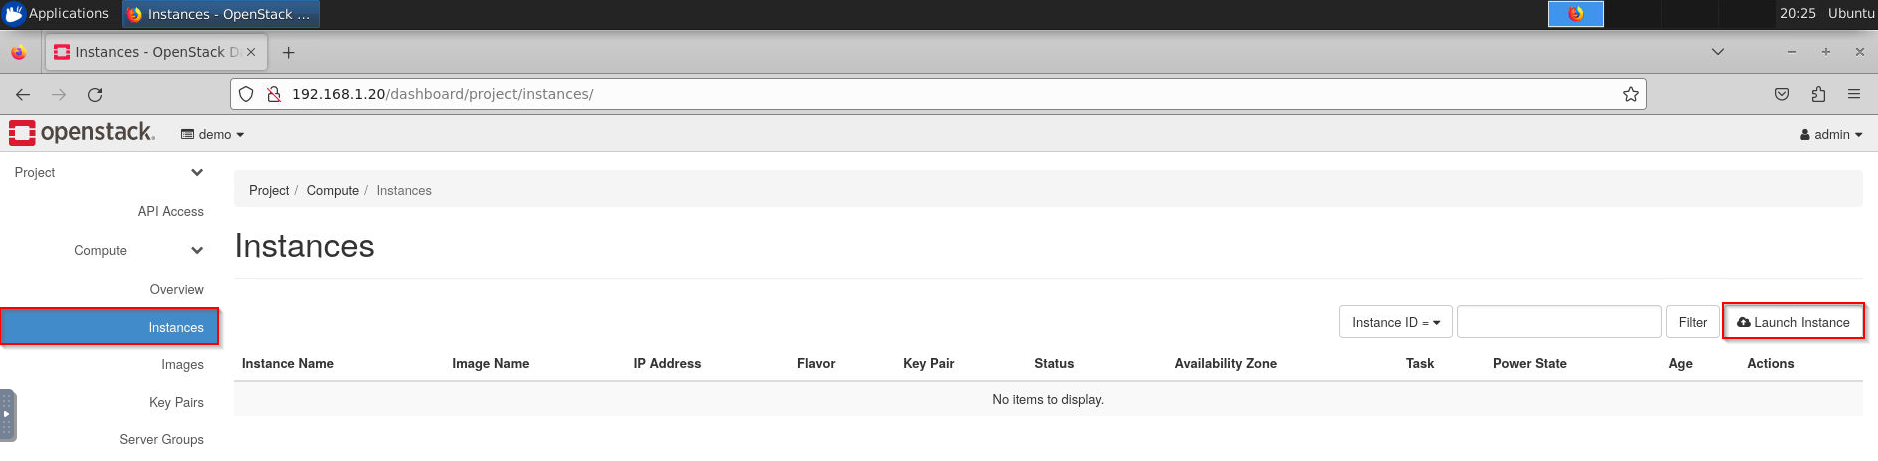
\includegraphics[width=\linewidth]{images/part1/step9.png}
    \end{center}

    \item In the \textit{Instance Name} field, type \textbf{prod-instance}, and leave the other fields with their
    default values. Click \textbf{Next}.

    \begin{center}
        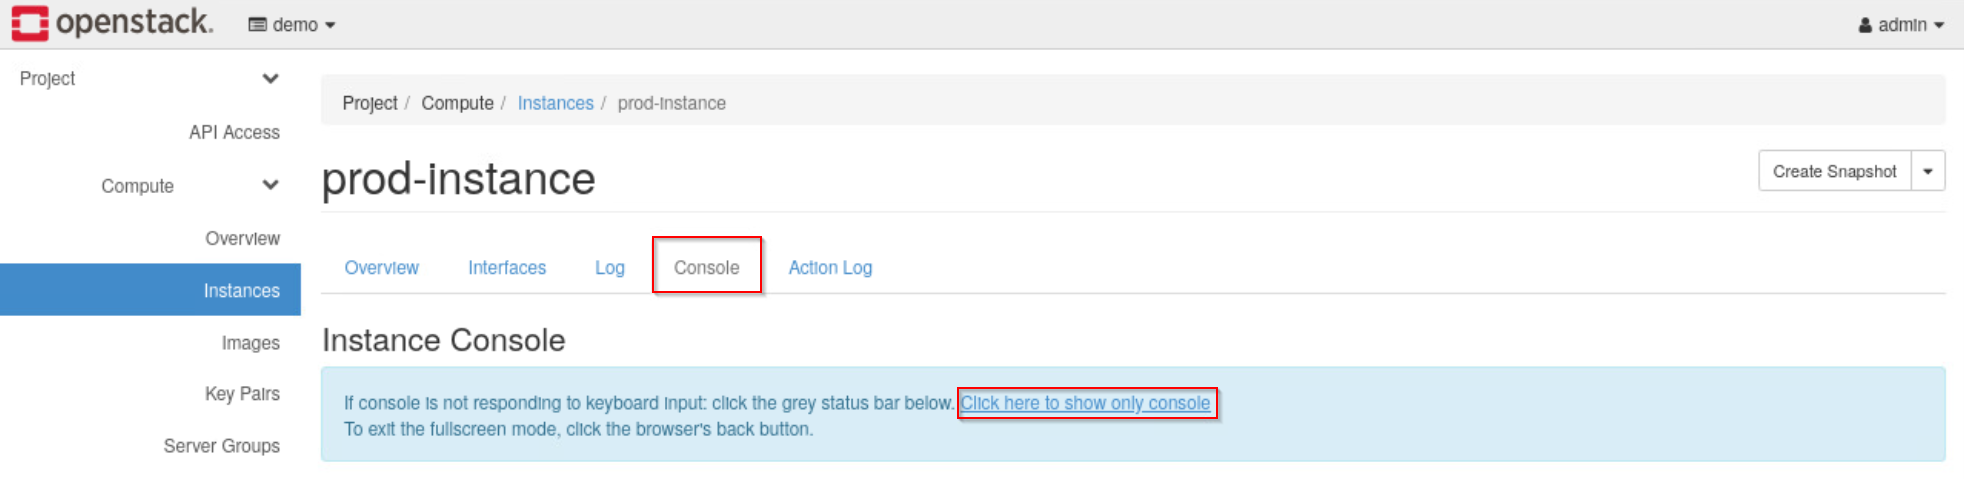
\includegraphics[width=\linewidth]{images/part1/step10.png}
    \end{center}

    \item In the \textit{Select Boot Source} drop dow, select \textbf{Image}, set \textit{Create New Volume} to
    \textbf{No} and scroll down (if needed) to click the $\uparrow$ icon beside of \textbf{cirros-0.6.2-x86-64-disk} to
    use \textbf{cirros-0.6.2-x86-64-disk} as the image. Click \textbf{Next}.

    \begin{center}
        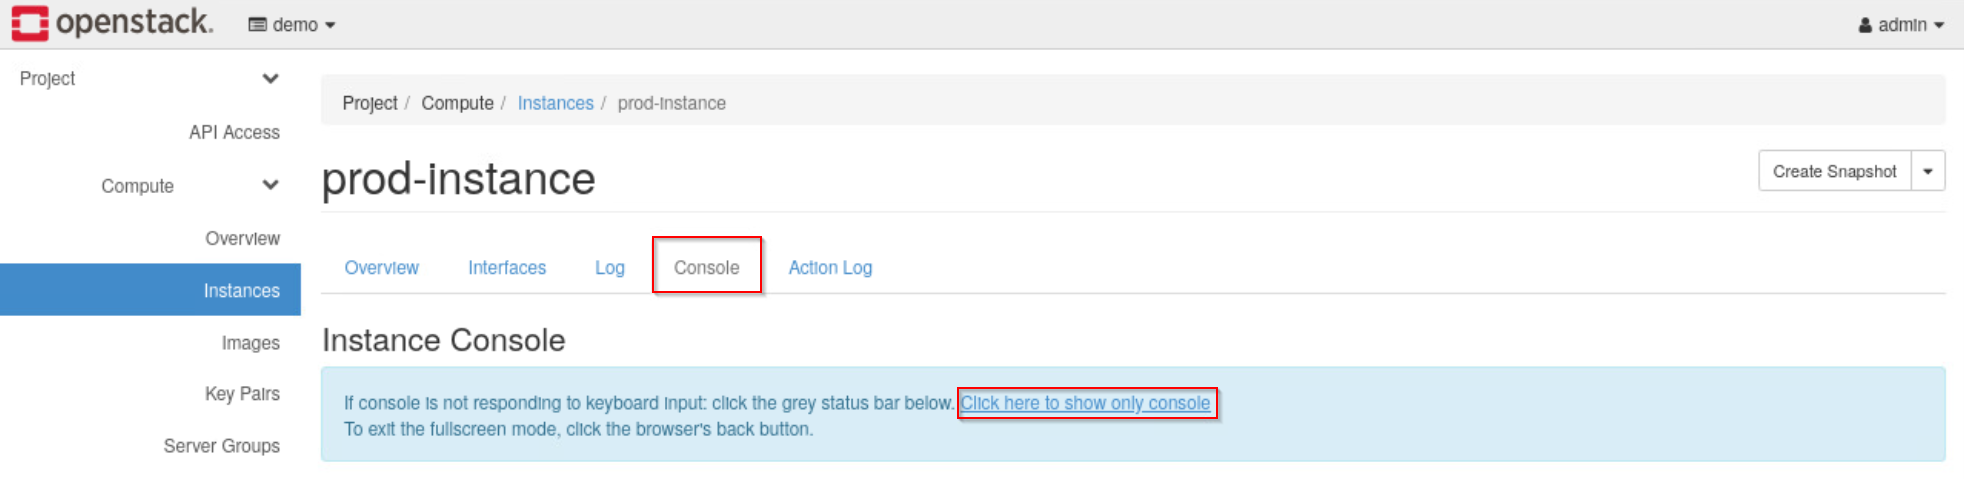
\includegraphics[width=\linewidth]{images/part1/step11.png}
    \end{center}

    \begin{stopbox}{}
        Before proceeding to the next step, confirm that \textbf{cirros-0.6.2-x86-64-disk} appears underneath the
        \textit{Allocated} section.
    \end{stopbox}
    
    \item Scroll down (if needed) and click the $\uparrow$ icon beside the \textbf{m1.tiny} flavor. Click \textbf{Next}.
    
    \begin{center}
        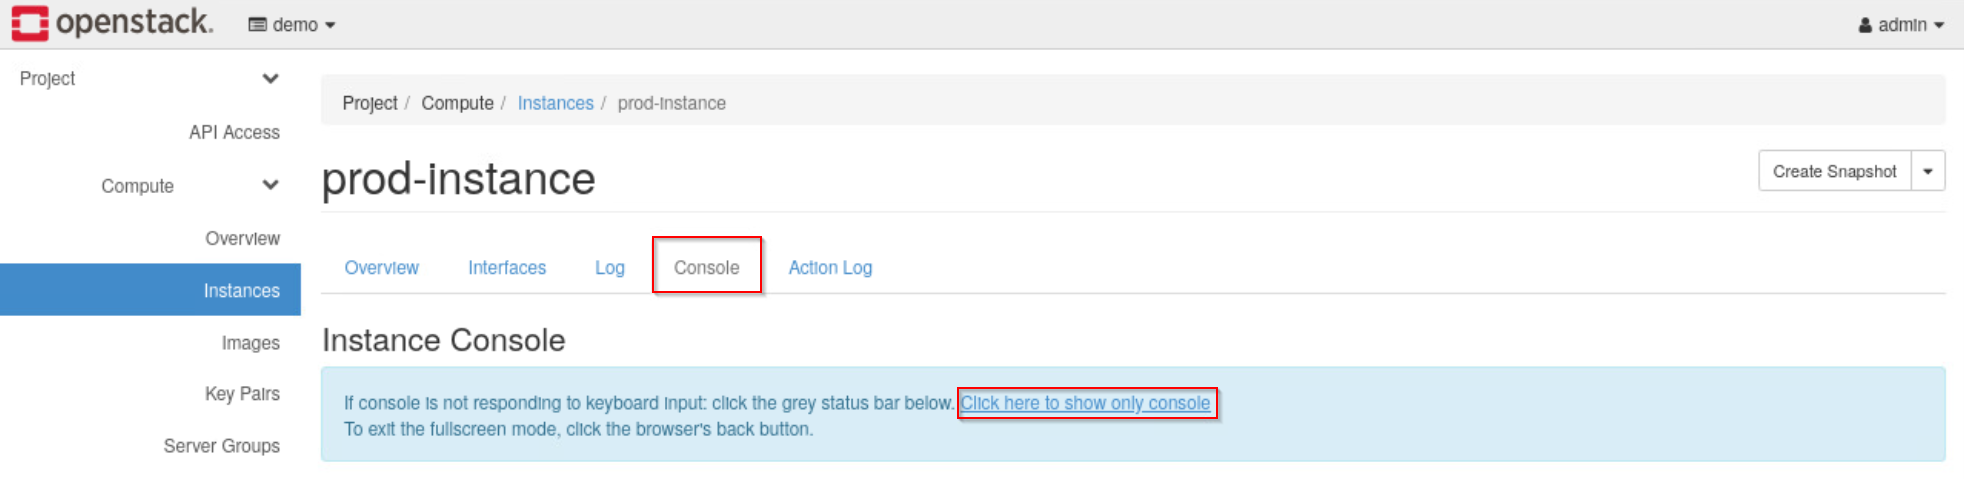
\includegraphics[width=\linewidth]{images/part1/step12.png}
    \end{center}

    \begin{stopbox}{}
        Before proceeding to the next step, confirm that \textbf{m1.tiny} appears underneath the \textit{Allocated}
        section.
    \end{stopbox}

    \item Click the $\uparrow$ icon beside the \textbf{shared} network. If all required fields have been set, the
    \textbf{Launch Instance} button in the bottom right corner should now be clickable. Click \textbf{Launch Instance}.

    \begin{center}
        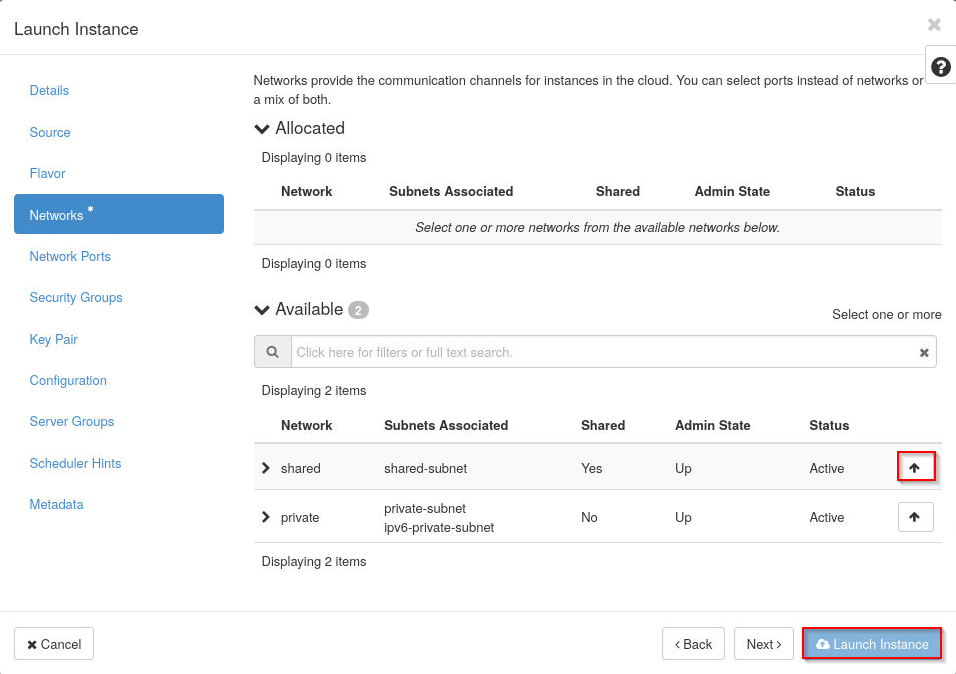
\includegraphics[width=\linewidth]{images/part1/step13.png}
    \end{center}

    \begin{stopbox}{}
        Before proceeding to the next step, confirm that \textbf{shared} appears underneath the \textit{Allocated}
        section.
    \end{stopbox}

    \item To open the conosle of \textbf{prod-instance} in a new tab, right-click on the name \textbf{prod-instance} and
    select \textbf{Open Link in New Tab}, or middle-click the name \textbf{prod-instance}.

    \begin{center}
        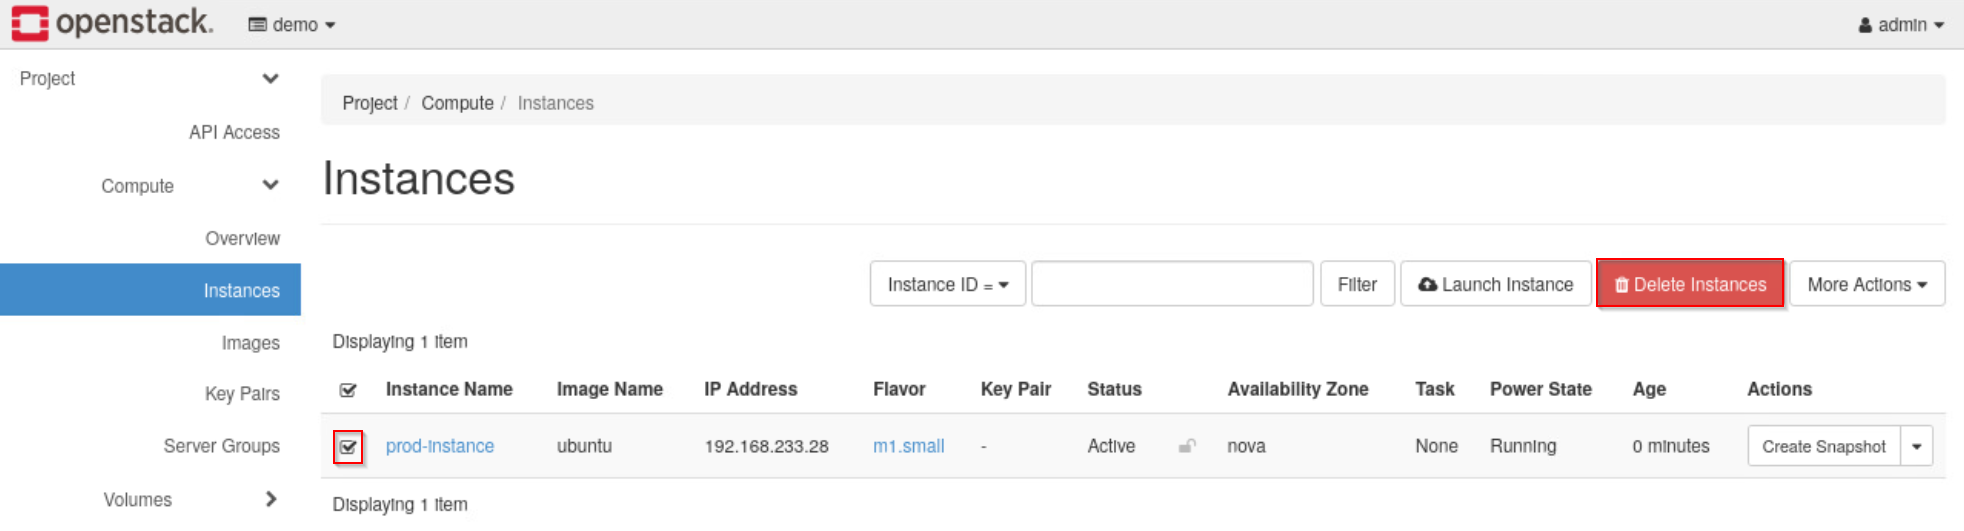
\includegraphics[width=\linewidth]{images/part1/step14.png}
    \end{center}

    \begin{stopbox}{}
        Wait for the \textit{Power State} of \textbf{prod-instance} to display the status of \textit{Running} before
        continuing to the next step.
    \end{stopbox}

    \item In the new tab, click the \textit{Console} tab. Optionally, to make the console take up the whole tab, click
    the \textbf{Click here to show only console} link.
    
    \begin{center}
        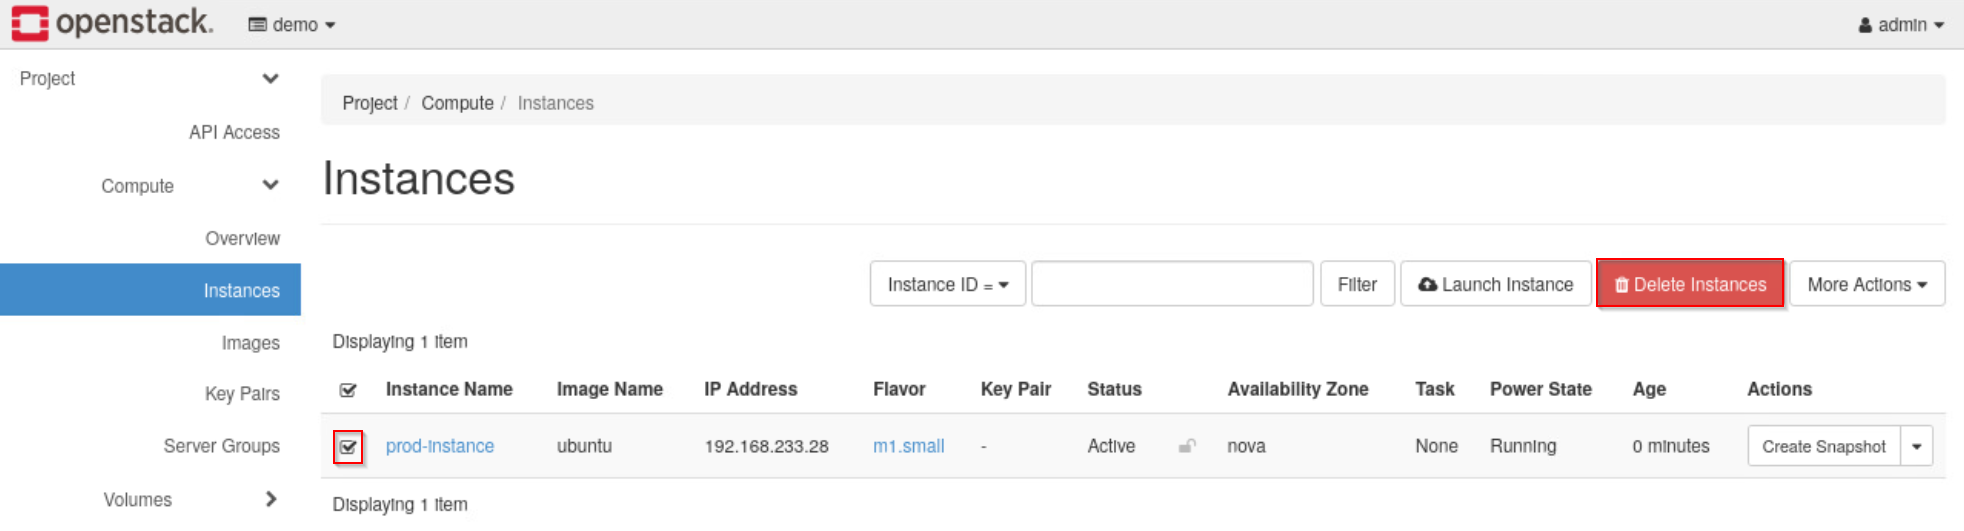
\includegraphics[width=\linewidth]{images/part1/step16.png}
    \end{center}

    \item Log into the console as \textbf{cirros} with password \textbf{gocubsgo}.

    \item In the console, ping \textbf{192.168.233.2} (DHCP server) to verify connectivity.
\begin{lstlisting}
$ ping -c3 192.168.233.2
\end{lstlisting}

    \begin{center}
        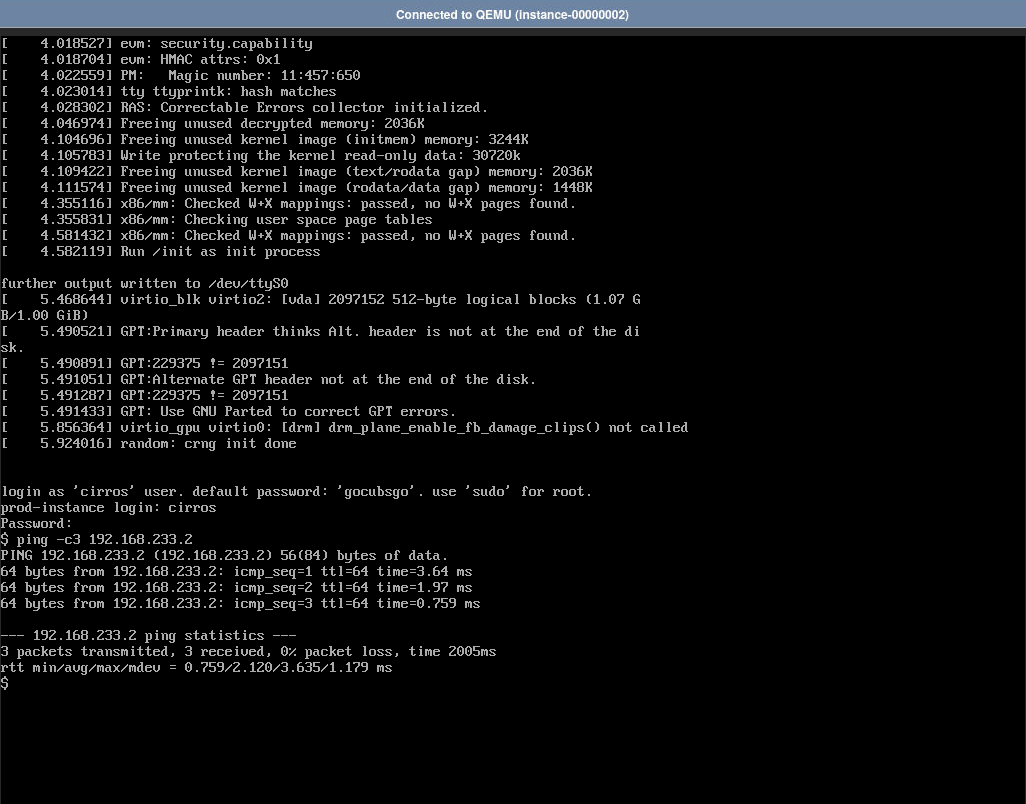
\includegraphics[width=\linewidth]{images/part1/step17.png}
    \end{center}

    \begin{notebox}{}
        You should have received three successful ping replies.
    \end{notebox}

    \item Close the console tab for \textbf{prod-instance}.

    \item Focus back on the tab showing instances and delete \textbf{prod-instance}. Select the checkbox for
    \textbf{prod-instance} and click the \textbf{Delete Instances} button.

    \begin{center}
        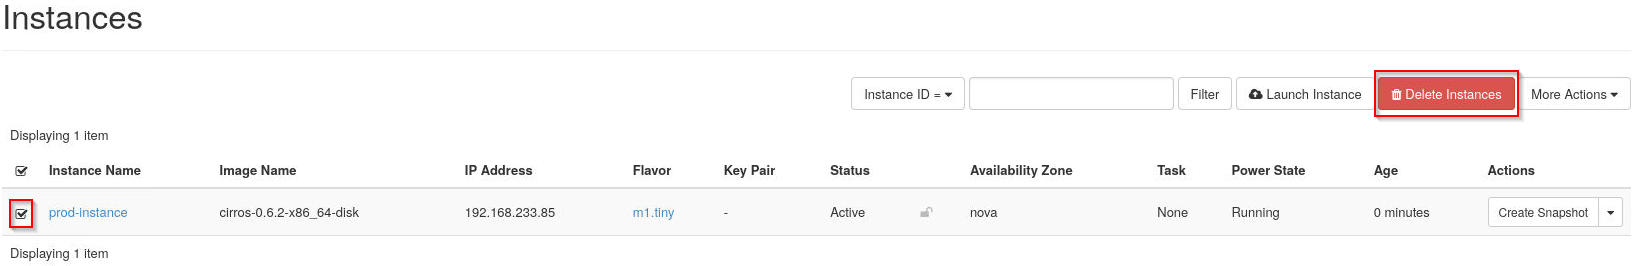
\includegraphics[width=\linewidth]{images/part1/step19.png}
    \end{center}

    \item Confirm the deletion by clicking the \textbf{Delete Instances} button.

    \begin{center}
        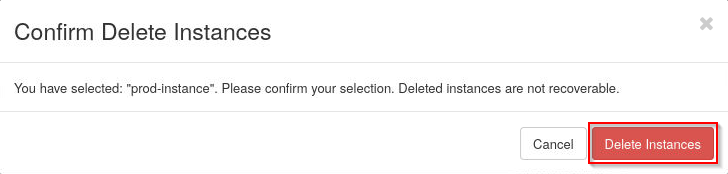
\includegraphics[width=\linewidth]{images/part1/step20.png}
    \end{center}

    \item Close the web browser.
\end{enumerate}

\section{Running the OpenStack Unified CLI}
In this task, you will use the \textit{OpenStack Unified command-line interface (CLI)} to list and check the details of
existing projects, users, flavors, images, and instances, and to launch an instance.

\begin{enumerate}
    \item Open a terminal, either by right-clicking the desktop and selecting \textbf{Open Terminal Here}, by clicking
    the terminal icon in the icon bar at the bottom of the screen, or by selecting \textbf{Applications} at the top
    left of the screen, then selecting \textbf{Terminal Emulator}.

    \begin{center}
        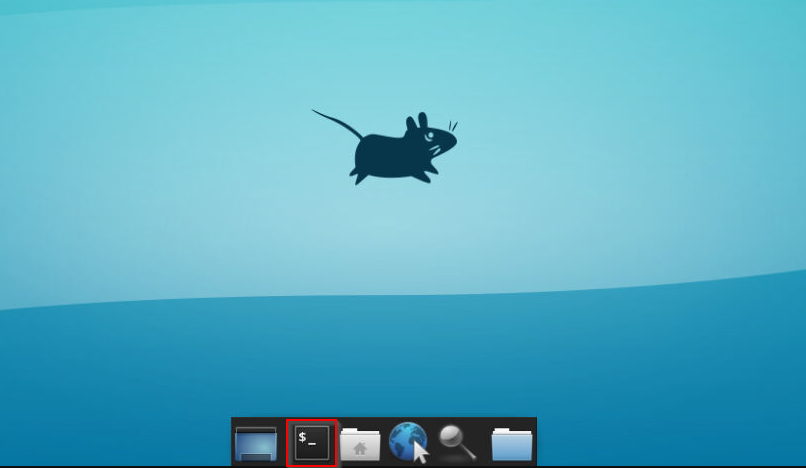
\includegraphics[width=\linewidth]{images/part2/step1.png}
    \end{center}

    \item Ensure you are in the home directory.
\begin{lstlisting}
ubuntu@workstation:/$ cd ~
\end{lstlisting}

    \begin{center}
        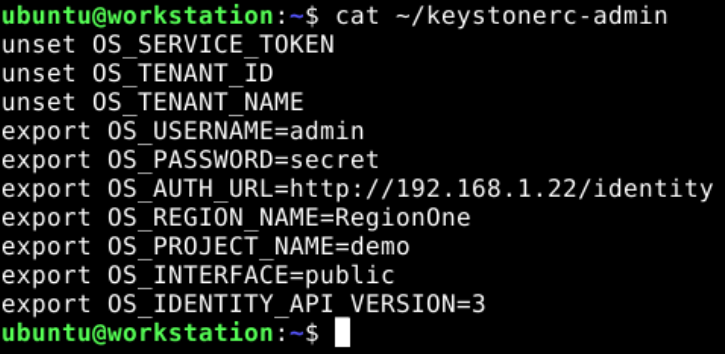
\includegraphics[width=\linewidth]{images/part2/step2.png}
    \end{center}

    \item The \textbf{keystonerc-admin} file in the home directory defines several \texttt{OS\_*} environment variables
    that allow you to use the OpenStack platform on the \textbf{devstack} server through the OpenStack Unified
    CLI. The username will be \textbf{admin}, the password will be be \textbf{secret}, the project will be
    \textbf{demo}, and the IP address for \texttt{OS\_AUTH\_URL} is the IP address of the \textbf{devstack} server,
    \textbf{192.168.1.20}. You can run \textbf{\texttt{cat}} on the file to view its contents.
\begin{lstlisting}
ubuntu@workstation:~$ cat keystonerc-admin
\end{lstlisting}

    \begin{center}
        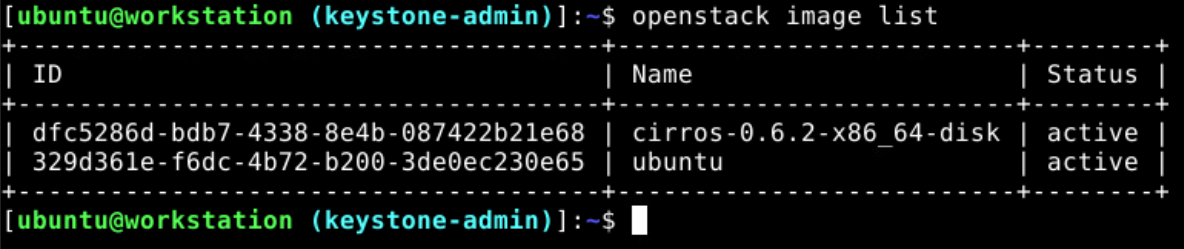
\includegraphics[width=\linewidth]{images/part2/step3.png}
    \end{center}

    \item Use the \textbf{\texttt{source}} command with the \textbf{keystonerc-admin} argument to enable all the
    \texttt{OS\_*} environment variables included in the \textbf{keystonerc-admin} file.
\begin{lstlisting}
ubuntu@workstation:~$ source keystonerc-admin
\end{lstlisting}

    \begin{center}
        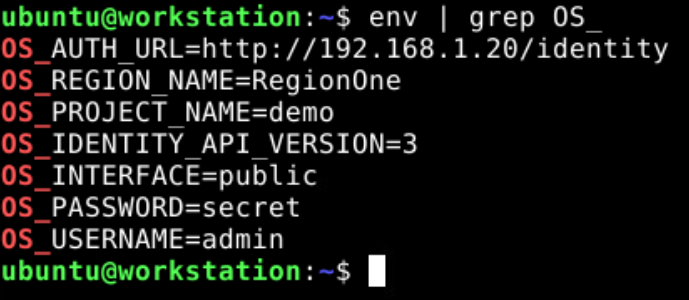
\includegraphics[width=\linewidth]{images/part2/step4.png}
    \end{center}

    \item Verify that the \texttt{OS\_*} environment variables have been exported to the shell environment.
\begin{lstlisting}
ubuntu@workstation:~$ env | grep OS_
\end{lstlisting}

    \begin{center}
        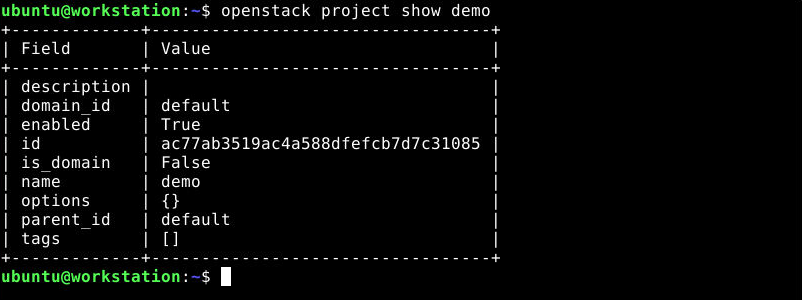
\includegraphics[width=\linewidth]{images/part2/step5.png}
    \end{center}

    \begin{tipbox}{}
        Use the \textbf{\texttt{openstack help project show}} command to determine how to display the details of a
        particular project.
    \end{tipbox}

    \item Enter the command below to gather additional information about the \textbf{admin} user's current project,
    \textbf{demo}.
\begin{lstlisting}
ubuntu@workstation:~$ openstack project show demo
\end{lstlisting}

    \begin{center}
        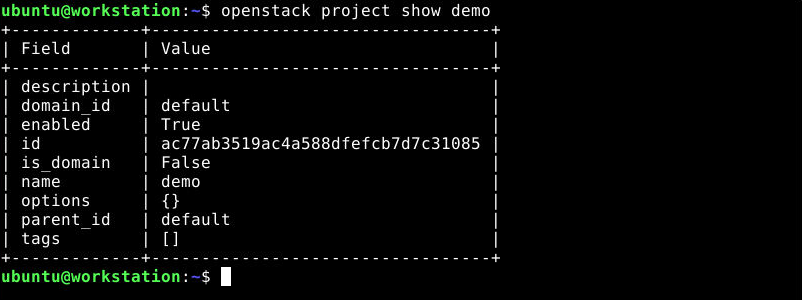
\includegraphics[width=\linewidth]{images/part2/step6.png}
    \end{center}

    \begin{notebox}
        The ID value for \textbf{demo} may differ from above since it is a unique ID.
    \end{notebox}

    \begin{tipbox}{}
        Use the \textbf{\texttt{openstack help user show}} command to determine how to display details of a specific
        user account.
    \end{tipbox}

    \item Enter the command below to check the details of \textbf{admin}.
\begin{lstlisting}
ubuntu@workstation:~$ openstack user show admin
\end{lstlisting}

    \begin{center}
        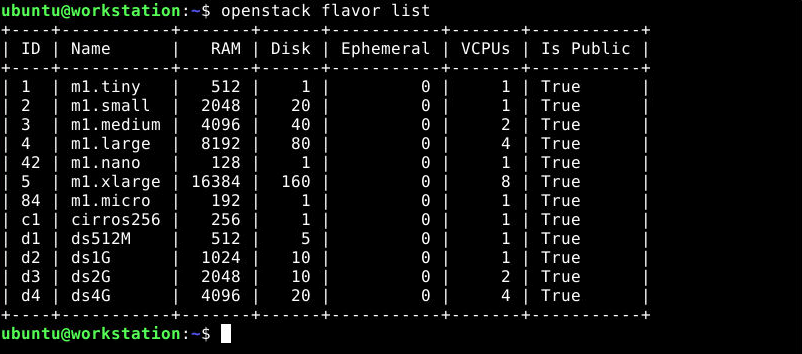
\includegraphics[width=\linewidth]{images/part2/step7.png}
    \end{center}

    \begin{tipbox}{}
        Use the \textbf{\texttt{openstack help flavor list}} command to determine how to display all available flavors.
    \end{tipbox}

    \item Enter the command below to list all available flavors.
\begin{lstlisting}
ubuntu@workstation:~$ openstack flavor list
\end{lstlisting}

    \begin{center}
        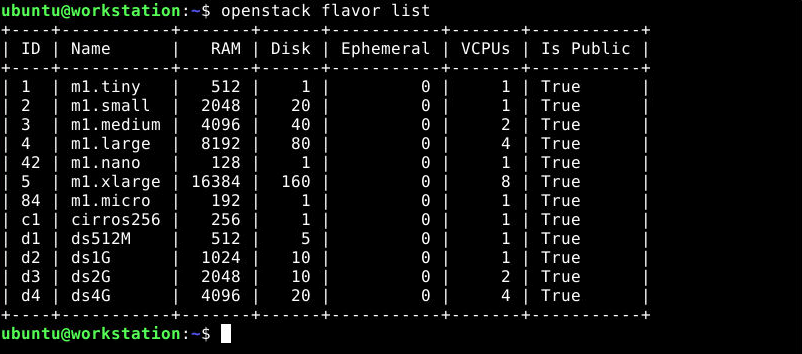
\includegraphics[width=\linewidth]{images/part2/step8.png}
    \end{center}

    \item Enter the command below to display the details specifically for the \textbf{m1.tiny} flavor.
\begin{lstlisting}
ubuntu@workstation:~$ openstack flavor show m1.tiny
\end{lstlisting}

    \begin{center}
        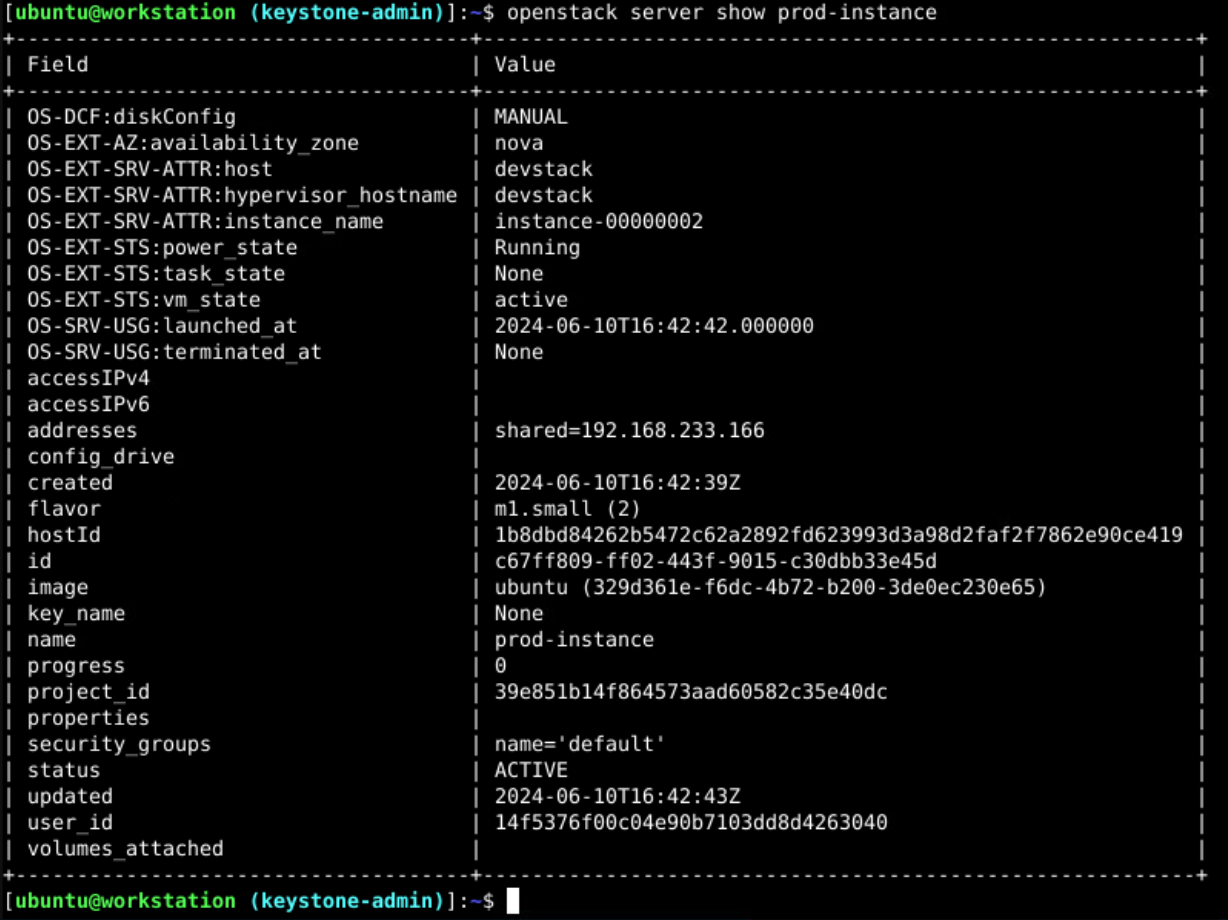
\includegraphics[width=\linewidth]{images/part2/step9.png}
    \end{center}

    \begin{tipbox}{}
        Use the \textbf{\texttt{openstack help image}} command to determine how to list all images.
    \end{tipbox}

    \item Enter the command below to list all available images.
\begin{lstlisting}
ubuntu@workstation:~$ openstack image list
\end{lstlisting}

    \begin{center}
        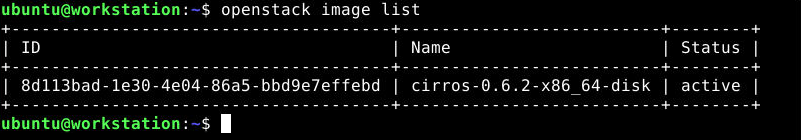
\includegraphics[width=\linewidth]{images/part2/step10.png}
    \end{center}

    \begin{tipbox}{}
        Use the \textbf{\texttt{openstack help network}} command to determine how to list all networks.
    \end{tipbox}

    \item Enter the command below to list all available networks.
\begin{lstlisting}
ubuntu@workstation:~$ openstack network list
\end{lstlisting}

    \begin{center}
        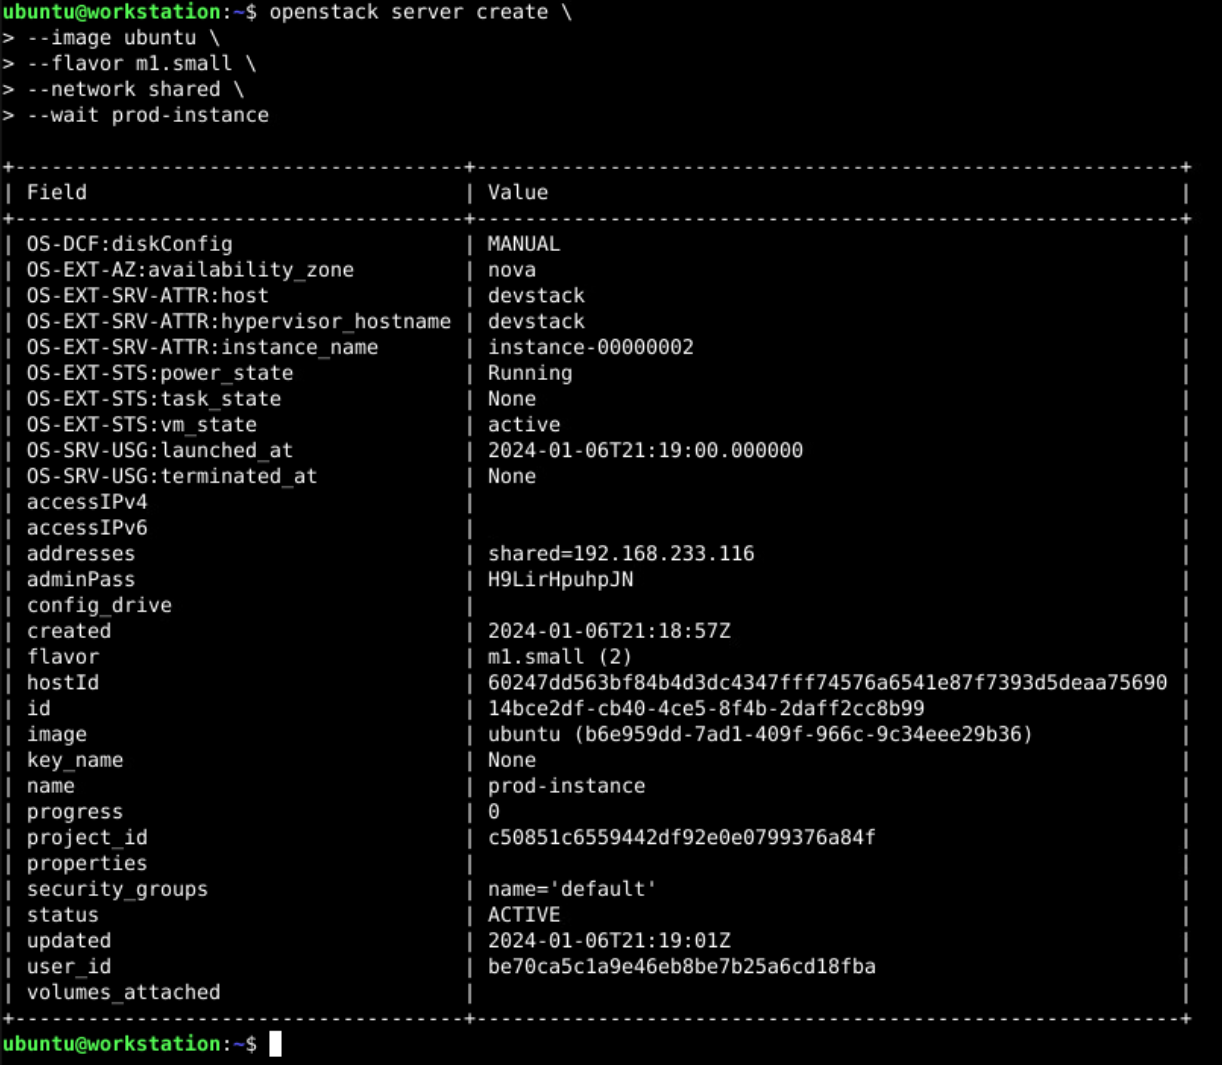
\includegraphics[width=\linewidth]{images/part2/step11.png}
    \end{center}

    \item Enter the command below to create a new instance with the name \textbf{prod-instance}, using
    \textbf{cirros-0.6.2-x86\_64-disk} as the image, \textbf{m1.tiny} as the flavor, and \textbf{shared} as the network.
\begin{lstlisting}
ubuntu@workstation:~$ openstack server create --image cirros-0.6.2-x86_64-disk \
> --flavor m1.tiny --network shared --wait prod-instance
\end{lstlisting}

    \begin{center}
        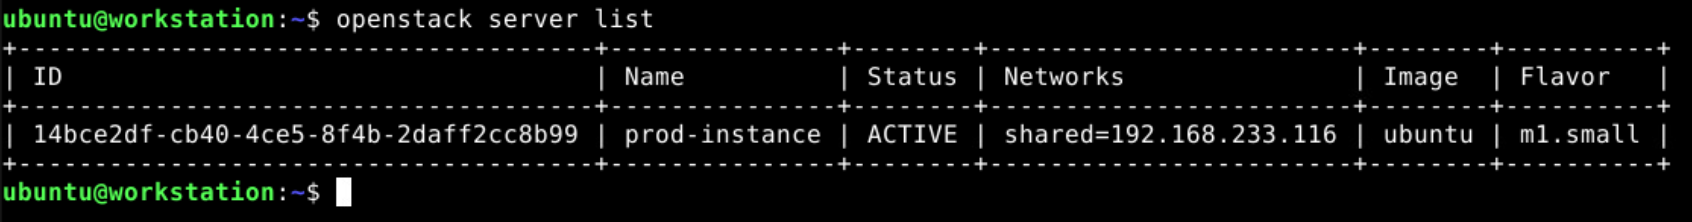
\includegraphics[width=\linewidth]{images/part2/step12.png}
    \end{center}

    \begin{tipbox}{}
        When typing the command, make sure there is a space between \texttt{cirros-0.6.2-x86\_64-disk} and the
        \texttt{\textbackslash}, and press \textbf{Enter} to get the \texttt{>} and continue typing the rest of the
        command.
    \end{tipbox}

    \item Use the \textbf{openstack server list} command to list all the available instances.
\begin{lstlisting}
ubuntu@workstation:~$ openstack server list
\end{lstlisting}

    \begin{center}
        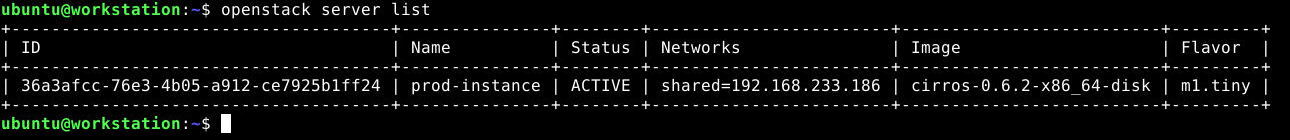
\includegraphics[width=\linewidth]{images/part2/step13.png}
    \end{center}

    \begin{notebox}{}
        The UUID in the \textit{ID} field and the IP address in the \textit{Networks} field may differ from the
        screenshot provided.
    \end{notebox}

    \item Enter the command below to display more details about the instance \textbf{prod-instance}.
\begin{lstlisting}
ubuntu@workstation:~$ openstack server show prod-instance
\end{lstlisting}

    \begin{center}
        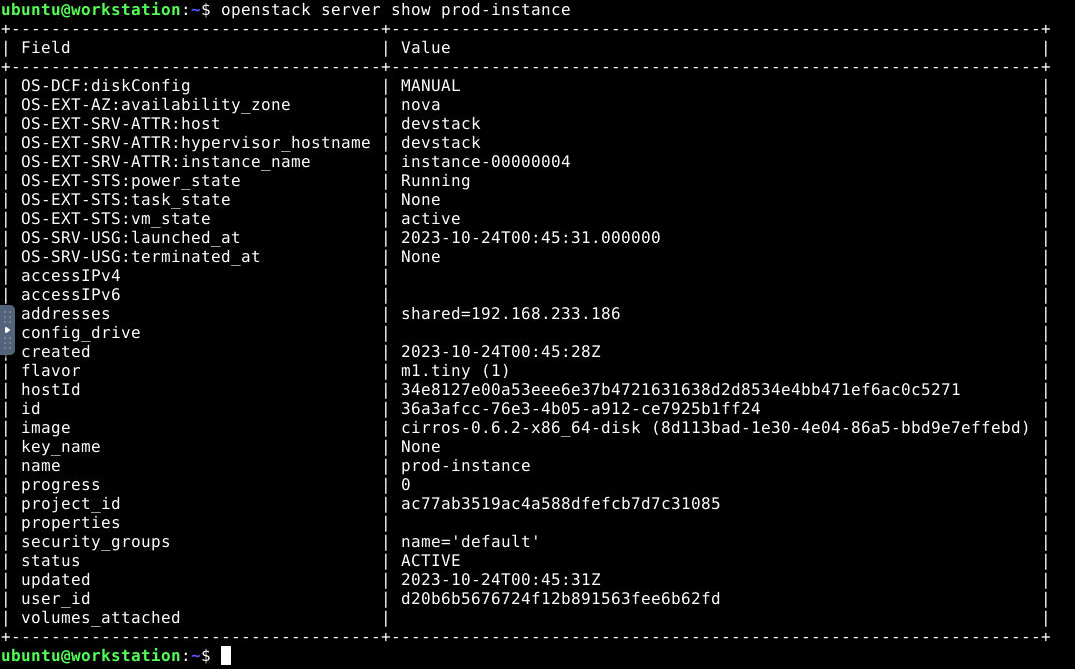
\includegraphics[width=\linewidth]{images/part2/step14.png}
    \end{center}

    \begin{tipbox}{}
        The UUID for the instance \textbf{prod-instance} can be used in place of \textbf{prod-instance} in the above
        command to identify the instance.
    \end{tipbox}

    \item Enter the command below to verify the log for the instance.
\begin{lstlisting}
ubuntu@workstation:~$ openstack console log show prod-instance
\end{lstlisting}

    \begin{center}
        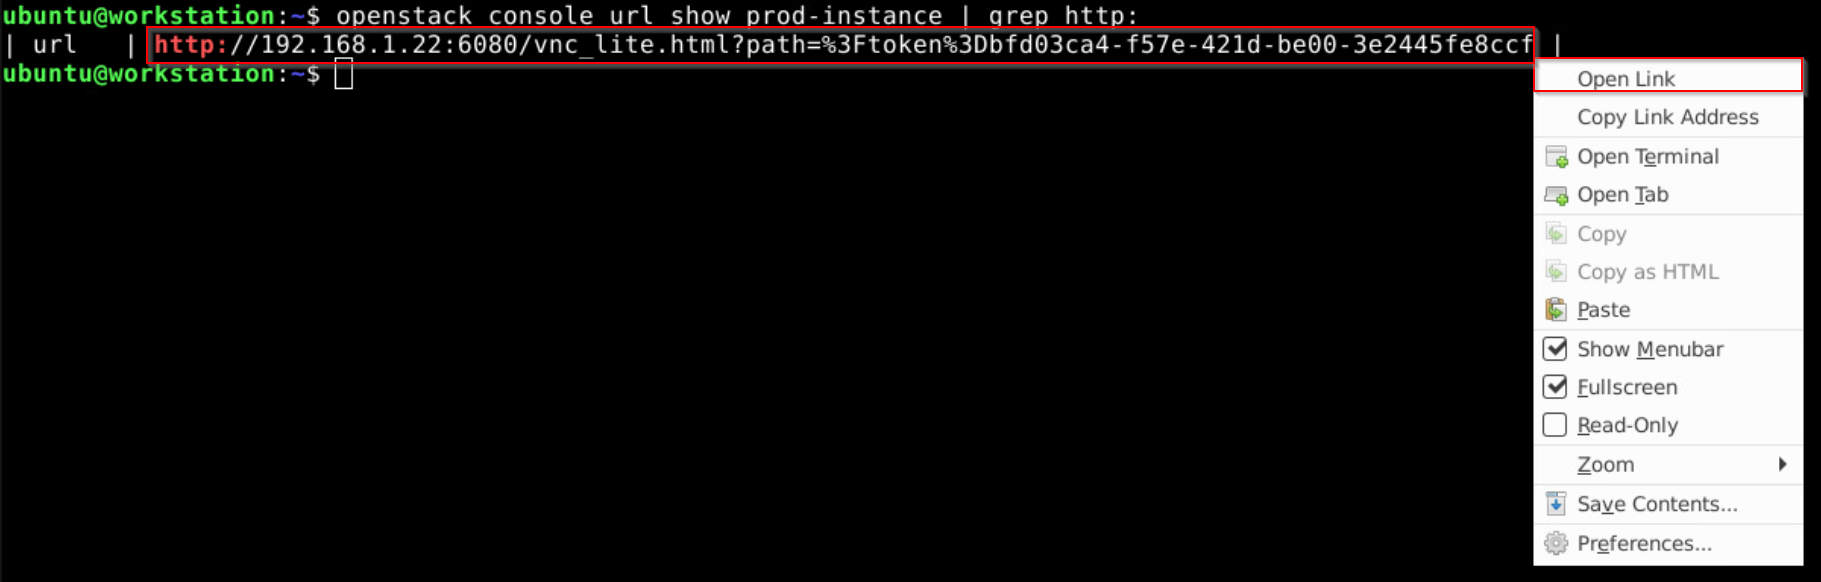
\includegraphics[width=\linewidth]{images/part2/step15.png}
    \end{center}

    \item Enter the command below to display the instance's console URL. Pipe the command to \textbf{\texttt{grep}} so
    that you will get a link in the terminal you can clikc on. Then right click on the URL and select \textbf{Open
    Link}.
\begin{lstlisting}
ubuntu@workstation:~$ openstack console url show prod-instance grep https:
\end{lstlisting}

    \begin{center}
        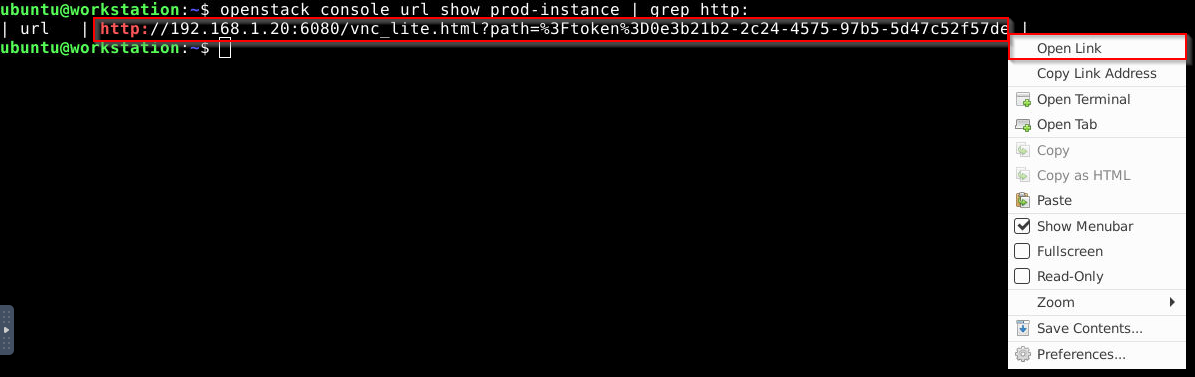
\includegraphics[width=\linewidth]{images/part2/step16.png}
    \end{center}

    \item The web browser will open directly to the instance's console through noVNC. Log into \textbf{prod-instance}
    using \textbf{cirros} as the username and \textbf{gocubsgo} as the password. Then use the \textbf{\texttt{ping}}
    command to verify connectivity with the DHCP server (\textbf{192.168.233.2}).
\begin{lstlisting}
$ ping -c3 192.168.233.2
\end{lstlisting}

    \begin{center}
        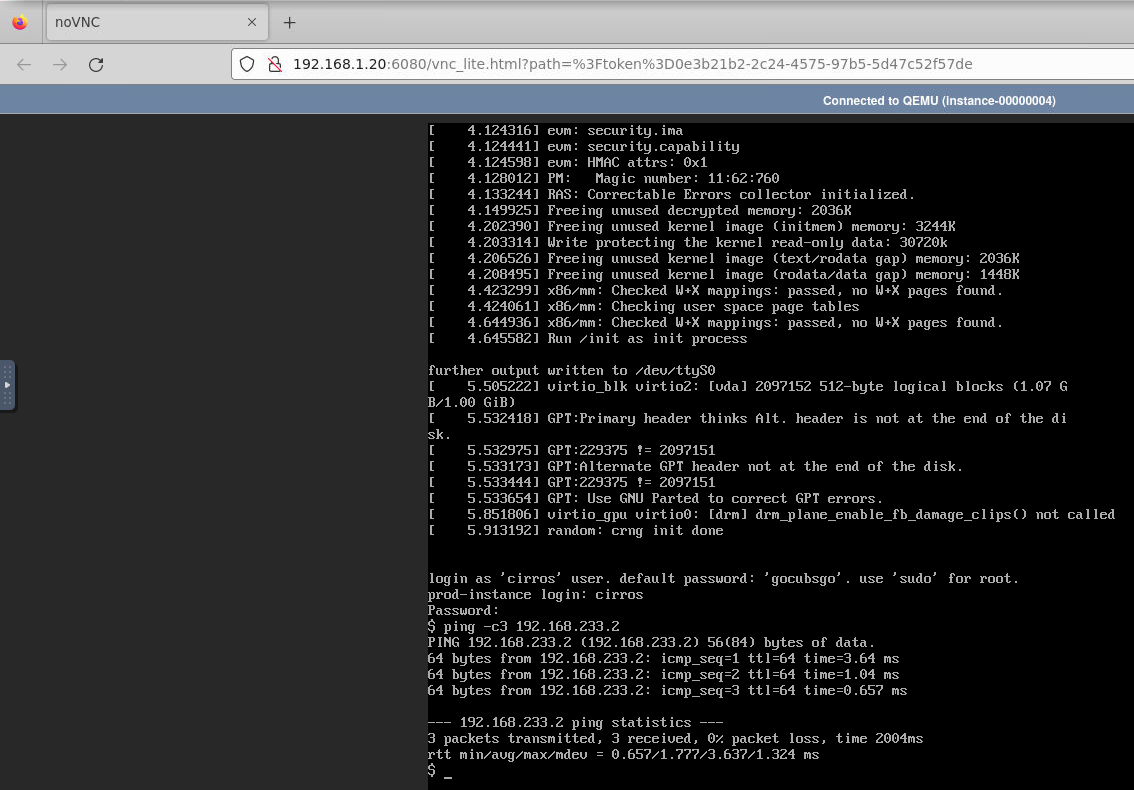
\includegraphics[width=\linewidth]{images/part2/step17.png}
    \end{center}

    \item Close the web browser and change focus back to the previous terminal window.
    
    \item Enter the command below to stop the instance
\begin{lstlisting}
ubuntu@workstation:~$ openstack server stop prod-instance
\end{lstlisting}

    \begin{center}
        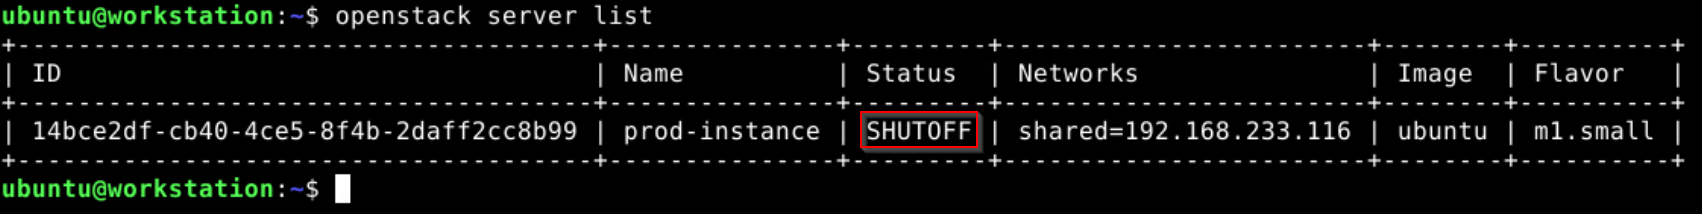
\includegraphics[width=\linewidth]{images/part2/step19.png}
    \end{center}

    \item \textbf{prod-instance} should now be in the \textbf{\texttt{SHUTOFF}} state. Enter the command below to verify this.
\begin{lstlisting}
ubuntu@workstation~$: openstack server list
\end{lstlisting}

    \begin{center}
        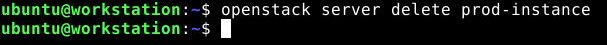
\includegraphics[width=\linewidth]{images/part2/step20.png}
    \end{center}

    \item Enter the command below to delete the instance.
\begin{lstlisting}
ubuntu@workstation:~$ openstack server delete prod-instance
\end{lstlisting}

    \begin{center}
        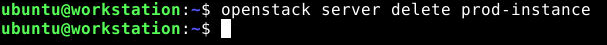
\includegraphics[width=\linewidth]{images/part2/step21.png}
    \end{center}

    \item The lab is now complete.

\end{enumerate}

\end{document}
